\documentclass[12pt, tikz, margin=1cm]{standalone}
\usepackage{xeCJK}
\usepackage{fontspec}
% \usepackage[a4paper,top=2.8cm,bottom=2.8cm,left=2.5cm,right=2.5cm, landscape]{geometry}
\usepackage{graphicx}
\usepackage{listings}
\usepackage{xcolor}
\usepackage{indentfirst}
\usepackage{tikz}
\usepackage{amssymb}
\usepackage{amsthm}
\usepackage{amsmath}
\usepackage{tabularx}
\usepackage{hyperref}
\usepackage{ulem}
\usepackage{version}
\usepackage{thmtools}
\usepackage{qtree}
\usepackage{algpseudocode}
\usepackage{mathtools}
% \usepackage[active,tightpage]{preview}
% \usepackage{varwidth}

\XeTeXlinebreaklocale "zh"
\XeTeXlinebreakskip = 0pt plus 1pt

\setCJKmainfont[BoldFont={SourceHanSerifTW-SemiBold.otf},AutoFakeSlant]{SourceHanSerifTW-Regular.otf}
\usetikzlibrary{arrows,decorations.markings,decorations.pathreplacing}

\tikzstyle {graph node} = [circle, draw, minimum width=1cm]
\tikzset{edge/.style = {decoration={markings,mark=at position 1 with %
            {\arrow[scale=2,>=stealth]{>}}},postaction={decorate}}}

\begin{document}

% \begin{preview}
% \begin{varwidth}{\linewidth}

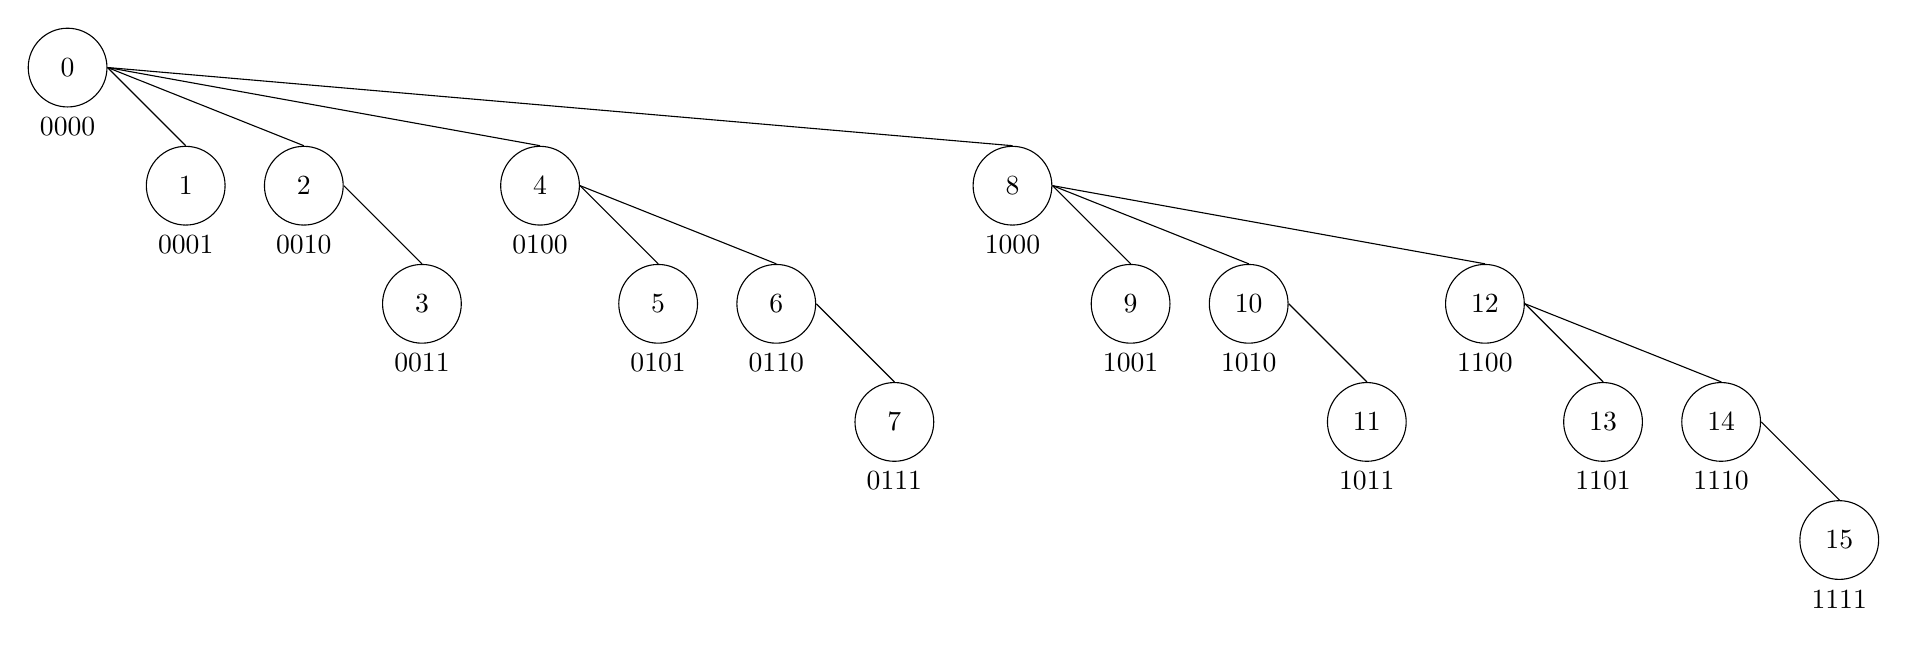
\begin{tikzpicture}[scale=1.5]
    \node[circle, draw, minimum width=1cm] (v0) at (0, 5) {0};
    \node[circle, draw, minimum width=1cm] (v1) at (1, 4) {1};
    \node[circle, draw, minimum width=1cm] (v2) at (2, 4) {2};
    \node[circle, draw, minimum width=1cm] (v4) at (4, 4) {4};
    \node[circle, draw, minimum width=1cm] (v8) at (8, 4) {8};
    \node[circle, draw, minimum width=1cm] (v3) at (3, 3) {3};
    \node[circle, draw, minimum width=1cm] (v5) at (5, 3) {5};
    \node[circle, draw, minimum width=1cm] (v6) at (6, 3) {6};
    \node[circle, draw, minimum width=1cm] (v9) at (9, 3) {9};
    \node[circle, draw, minimum width=1cm] (v10) at (10, 3) {10};
    \node[circle, draw, minimum width=1cm] (v12) at (12, 3) {12};
    \node[circle, draw, minimum width=1cm] (v7) at (7, 2) {7};
    \node[circle, draw, minimum width=1cm] (v11) at (11, 2) {11};
    \node[circle, draw, minimum width=1cm] (v13) at (13, 2) {13};
    \node[circle, draw, minimum width=1cm] (v14) at (14, 2) {14};
    \node[circle, draw, minimum width=1cm] (v15) at (15, 1) {15};

    \node at (0, 5-0.5) {0000};
    \node at (1, 4-0.5) {0001};
    \node at (2, 4-0.5) {0010};
    \node at (4, 4-0.5) {0100};
    \node at (8, 4-0.5) {1000};
    \node at (3, 3-0.5) {0011};
    \node at (5, 3-0.5) {0101};
    \node at (6, 3-0.5) {0110};
    \node at (9, 3-0.5) {1001};
    \node at (10, 3-0.5) {1010};
    \node at (12, 3-0.5) {1100};
    \node at (7, 2-0.5) {0111};
    \node at (11, 2-0.5) {1011};
    \node at (13, 2-0.5) {1101};
    \node at (14, 2-0.5) {1110};
    \node at (15, 1-0.5) {1111};

    \draw (v0.east) -- (v1.north);
    \draw (v0.east) -- (v2.north);
    \draw (v0.east) -- (v4.north);
    \draw (v0.east) -- (v8.north);
    \draw (v2.east) -- (v3.north);
    \draw (v4.east) -- (v5.north);
    \draw (v4.east) -- (v6.north);
    \draw (v6.east) -- (v7.north);
    \draw (v8.east) -- (v9.north);
    \draw (v8.east) -- (v10.north);
    \draw (v8.east) -- (v12.north);
    \draw (v10.east) -- (v11.north);
    \draw (v12.east) -- (v13.north);
    \draw (v12.east) -- (v14.north);
    \draw (v14.east) -- (v15.north);
\end{tikzpicture}

% \end{varwidth}
% \end{preview}

\end{document}